\section{Satisfied\-IND$<$ Data $>$ Class Template Reference}
\label{class_satisfied_i_n_d}\index{SatisfiedIND@{SatisfiedIND}}
Functor representing the predicate being a satisfied {\bf IND}{\rm (p.\,\pageref{class_i_n_d})} wrt to 2 relations.  


{\tt \#include $<$Satisfied\-IND.hxx$>$}

Inheritance diagram for Satisfied\-IND$<$ Data $>$::\begin{figure}[H]
\begin{center}
\leavevmode
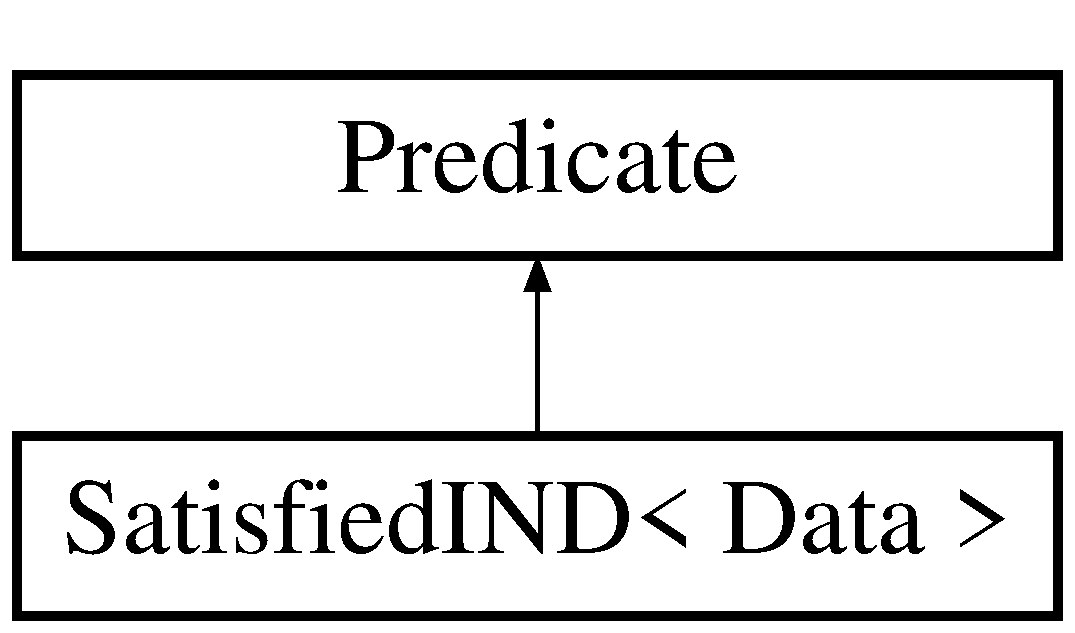
\includegraphics[height=2cm]{class_satisfied_i_n_d}
\end{center}
\end{figure}
\subsection*{Public Member Functions}
\begin{CompactItemize}
\item 
template$<$class Input\-DBFormat$>$ {\bf Satisfied\-IND} (Data \&intable1, Input\-DBFormat \&input1, Data \&intable2, Input\-DBFormat \&input2)
\begin{CompactList}\small\item\em Constructor. \item\end{CompactList}\item 
{\bf $\sim$Satisfied\-IND} ()\label{class_satisfied_i_n_d_42ee5fbb4365e4ebaa5b6d2811cd90a5}

\begin{CompactList}\small\item\em Destructor. \item\end{CompactList}\item 
template$<$class Iterator, class Measure$>$ bool {\bf operator()} (Iterator it\-Cand, Measure \&mes\-Cand)
\begin{CompactList}\small\item\em Operator that test if a set of attributes is a satisfied {\bf IND}{\rm (p.\,\pageref{class_i_n_d})}. \item\end{CompactList}\end{CompactItemize}
\subsection*{Protected Member Functions}
\begin{CompactItemize}
\item 
template$<$class Container\-Attrib, class Container\-Project$>$ void {\bf projection} (Data $\ast$relation, Container\-Attrib \&set\-Of\-Attrib, Container\-Project \&project, {\bf Recode\-To\-Int}$<$ string $>$ \&num\-Attrib)
\begin{CompactList}\small\item\em function used to project a relation wrt a set of attributes. \item\end{CompactList}\end{CompactItemize}
\subsection*{Protected Attributes}
\begin{CompactItemize}
\item 
Data $\ast$ {\bf table1}\label{class_satisfied_i_n_d_40870e6e2f4d671c3658f4e9d9775b70}

\begin{CompactList}\small\item\em the first relation 1 \item\end{CompactList}\item 
Data $\ast$ {\bf table2}\label{class_satisfied_i_n_d_067ee67848d21e1bc5f04f1531e60a51}

\begin{CompactList}\small\item\em the first relation 2 \item\end{CompactList}\item 
{\bf Recode\-To\-Int}$<$ string $>$ {\bf num\-Attrib1}\label{class_satisfied_i_n_d_2e89ec65c6746fba9dc90eda29197867}

\begin{CompactList}\small\item\em Used to get the numero of the attributes ( 1st, 2nd,...) of the first relation. \item\end{CompactList}\item 
{\bf Recode\-To\-Int}$<$ string $>$ {\bf num\-Attrib2}\label{class_satisfied_i_n_d_01f0ff69e35875dbc6b9c02f7b514fc4}

\begin{CompactList}\small\item\em Used to get the numero of the attributes ( 1st, 2nd,...) of the first relation. \item\end{CompactList}\end{CompactItemize}
\subsection*{Classes}
\begin{CompactItemize}
\item 
class {\bf Process\-Tuples}
\begin{CompactList}\small\item\em Functor used to projet all the tuples wrt attributes studied. \item\end{CompactList}\item 
class {\bf project2}
\begin{CompactList}\small\item\em Functor used to projet a tuple wrt the set of attributes studied. \item\end{CompactList}\end{CompactItemize}


\subsection{Detailed Description}
\subsubsection*{template$<$class Data$>$ class Satisfied\-IND$<$ Data $>$}

Functor representing the predicate being a satisfied {\bf IND}{\rm (p.\,\pageref{class_i_n_d})} wrt to 2 relations. 

This functor test if a {\bf IND}{\rm (p.\,\pageref{class_i_n_d})} is satisfied. The method used to test if a candidate is a a satisfied {\bf IND}{\rm (p.\,\pageref{class_i_n_d})} is the following one: process the projection wrt the attributes of the left side of the candidate {\bf IND}{\rm (p.\,\pageref{class_i_n_d})}. process the projection wrt the attributes of the right side of the candidate {\bf IND}{\rm (p.\,\pageref{class_i_n_d})}. check that each element of left side projection is included in the right side projection. return true if all the element are included.

The template parameter Data is the type of the tablular data. 



\subsection{Constructor \& Destructor Documentation}
\index{SatisfiedIND@{Satisfied\-IND}!SatisfiedIND@{SatisfiedIND}}
\index{SatisfiedIND@{SatisfiedIND}!SatisfiedIND@{Satisfied\-IND}}
\subsubsection{\setlength{\rightskip}{0pt plus 5cm}template$<$class Data$>$ template$<$class Input\-DBFormat$>$ {\bf Satisfied\-IND}$<$ Data $>$::{\bf Satisfied\-IND} (Data \& {\em intable1}, Input\-DBFormat \& {\em input1}, Data \& {\em intable2}, Input\-DBFormat \& {\em input2})\hspace{0.3cm}{\tt  [inline]}}\label{class_satisfied_i_n_d_083227d8e372ee6954f7e11e5c84d4bc}


Constructor. 

\begin{Desc}
\item[Parameters:]
\begin{description}
\item[{\em intable1}]data of the first relation/table studied \item[{\em input1}]file containing the first relation/table studied \item[{\em intable2}]data of the second relation/table studied \item[{\em input2}]file containing the second relation/table studied \end{description}
\end{Desc}


\subsection{Member Function Documentation}
\index{SatisfiedIND@{Satisfied\-IND}!operator()@{operator()}}
\index{operator()@{operator()}!SatisfiedIND@{Satisfied\-IND}}
\subsubsection{\setlength{\rightskip}{0pt plus 5cm}template$<$class Data$>$ template$<$class Iterator, class Measure$>$ bool {\bf Satisfied\-IND}$<$ Data $>$::operator() (Iterator {\em it\-Cand}, Measure \& {\em mes\-Cand})}\label{class_satisfied_i_n_d_bbf69fd5dfbf71f8e7f0685b80551c6d}


Operator that test if a set of attributes is a satisfied {\bf IND}{\rm (p.\,\pageref{class_i_n_d})}. 

\begin{Desc}
\item[Parameters:]
\begin{description}
\item[{\em it\-Cand}]iterator (or pointer) on the set of attributes to test wrt the predicate \item[{\em mes\-Cand}]cardinality of the projection on the db of the attributes \end{description}
\end{Desc}


Reimplemented from {\bf Predicate} {\rm (p.\,\pageref{class_predicate_6fb1a75dba2268f75738f335f403e46c})}.\index{SatisfiedIND@{Satisfied\-IND}!projection@{projection}}
\index{projection@{projection}!SatisfiedIND@{Satisfied\-IND}}
\subsubsection{\setlength{\rightskip}{0pt plus 5cm}template$<$class Data$>$ template$<$class Container\-Attrib, class Container\-Project$>$ void {\bf Satisfied\-IND}$<$ Data $>$::projection (Data $\ast$ {\em relation}, Container\-Attrib \& {\em set\-Of\-Attrib}, Container\-Project \& {\em project}, {\bf Recode\-To\-Int}$<$ string $>$ \& {\em num\-Attrib})\hspace{0.3cm}{\tt  [protected]}}\label{class_satisfied_i_n_d_bb4eeaeb80e39c8e6dcc804444a1c44e}


function used to project a relation wrt a set of attributes. 

\begin{Desc}
\item[Parameters:]
\begin{description}
\item[{\em relation}]class representing the relation. \item[{\em Container\-Attrib}]set of attribute used for the projection. \item[{\em Container\-Project}]container used to store the projection. \end{description}
\end{Desc}


The documentation for this class was generated from the following file:\begin{CompactItemize}
\item 
F:/i\-Zi/problems/DI/Satisfied\-IND.hxx\end{CompactItemize}
